\documentclass[10pt, mathserif, profesionalfont]{beamer}

\usepackage[utf8]{inputenc}
\usepackage[spanish]{babel}



\usepackage{amsmath,amsfonts,amssymb,amsthm}
\usepackage{booktabs}
\usepackage{hyperref}
\usepackage{authblk}

\usepackage[acronym]{glossaries}

\renewcommand\Affilfont{\itshape\small}
\renewcommand\Authand{ y }

\newtheorem{thm}{Teorema}

\usepackage{array}
\newcolumntype{L}[1]{>{\raggedright\let\newline\\\arraybackslash\hspace{0pt}}p{#1}}
\newcolumntype{C}[1]{>{\centering\let\newline\\\arraybackslash\hspace{0pt}}p{#1}}
\newcolumntype{R}[1]{>{\raggedleft\let\newline\\\arraybackslash\hspace{0pt}}p{#1}}

\newcolumntype{X}[1]{>{\raggedright\let\newline\\\arraybackslash\hspace{0pt}}m{#1}}
\newcolumntype{Y}[1]{>{\centering\let\newline\\\arraybackslash\hspace{0pt}}m{#1}}
\newcolumntype{Z}[1]{>{\raggedleft\let\newline\\\arraybackslash\hspace{0pt}}m{#1}}

\usepackage{color}
\makeglossaries

\newacronym{ndtm}{NDTM}{Máquina de Turing No Determinista}

\newacronym{sat}{SAT}{SATISFACTIBILIDAD}

\newacronym{3dm}{3DM}{3-DimentionalMatching}



% There are many different themes available for Beamer. A comprehensive
% list with examples is given here:
% http://deic.uab.es/~iblanes/beamer_gallery/index_by_theme.html
% You can uncomment the themes below if you would like to use a different
% one:
%\usetheme{AnnArbor}
%\usetheme{Antibes}
%\usetheme{Bergen}
%\usetheme{Berkeley}
%\usetheme{Berlin}
%\usetheme{Boadilla}
%\usetheme{boxes}
%\usetheme{CambridgeUS}
\usetheme{Copenhagen}
%\usetheme{Darmstadt}
%\usetheme{default}
%\usetheme{Frankfurt}
%\usetheme{Goettingen}
%\usetheme{Hannover}
%\usetheme{Ilmenau}
%\usetheme{JuanLesPins}
%\usetheme{Luebeck}
%\usetheme{Madrid}
%\usetheme{Malmoe}
%\usetheme{Marburg}
%\usetheme{Montpellier}
%\usetheme{PaloAlto}
%\usetheme{Pittsburgh}
%\usetheme{Rochester}
%\usetheme{Singapore}
%\usetheme{Szeged}
%\usetheme{Warsaw}

\title{3-DIMENSIONAL MATCHING}

% A subtitle is optional and this may be deleted
\subtitle{Problema básico $\mathcal{NP}$-completo}

\author{Diego Luis Afonso \and Daniel Daher Pérez \and Cristina Tosco González \and Alberto Antonio Sarabia Suarez \and Daniel Antonio Fernández Pérez}
% - Give the names in the same order as the appear in the paper.
% - Use the \inst{?} command only if the authors have different
%   affiliation.

\institute[ULL-ESIT-Escuela Superior de Ingeniería y Tecnología]{Universidad de La Laguna} % (optional, but mostly needed)

% - Use the \inst command only if there are several affiliations.
% - Keep it simple, no one is interested in your street address.

\date{Curso 2016/2017}
% - Either use conference name or its abbreviation.
% - Not really informative to the audience, more for people (including
%   yourself) who are reading the slides online

\subject{Complejidad Computacional}
% This is only inserted into the PDF information catalog. Can be left
% out. 

% If you have a file called "university-logo-filename.xxx", where xxx
% is a graphic format that can be processed by latex or pdflatex,
% resp., then you can add a logo as follows:

% \pgfdeclareimage[height=0.5cm]{university-logo}{university-logo-filename}
% \logo{\pgfuseimage{university-logo}}

% Delete this, if you do not want the table of contents to pop up at
% the beginning of each subsection:
\AtBeginSubsection[]
{
	\begin{frame}<beamer>{Outline}
		\tableofcontents[currentsection,currentsubsection]
	\end{frame}
}

% Let's get started
\begin{document}
	
	\begin{frame}
		\titlepage
	\end{frame}
	
	
	
	
	\section{Introducción}
	
	\begin{frame}{Índice}
		
		\begin{enumerate}[1.]
			\item NP-Problem
			\item Clasificación NP-Problems
			\item Clasificación NP-Completitud
			\item Definición 3 - Dimentional Matching
			\begin{enumerate}[a)]
				\item Caso general
				\item Problema decisión
				\item Problema optimización
				\item Ejemplo
			\end{enumerate}
			\item Demostración 3 - Dimentional Matching es NP-Problem
			\item Demostración 3 - Dimentional Matching es NP-Completo
			\item Comparación grafo bipartito
		\end{enumerate}
		
	\end{frame}
	
	
	\begin{frame}{NP-Problems}
		\begin{block}{}
			\begin{itemize}
				\item Un problema se asigna a la clase {\textbf{NP}} (nondeterministic polynomial time - tiempo polinómico no determinista) si es resoluble en tiempo polinómico 
				por una {\textbf{Máquina de Turing}} no determinista.
				
				\item Gran cantidad de programas no (necesariamente) se ejecutan en tiempo polinómico en un PC, 
				pero se ejecuta en tiempo polinómico en una máquina de Turing no determinista.
				
				\item Estos programas resuelven {\textbf{problemas en NP}}.   
			\end{itemize}	
		\end{block}
		
		\begin{block}{}
			Todos los problemas en {\textbf{P están también en NP}}, es decir, una máquina de Turing no determinista puede hacer todo lo que un ordenador normal puede y más.
		\end{block}
	\end{frame}
	
	
	\begin{frame}{NP-Problems I}
		\begin{block}{Definición equivalente NP-Problem}
			Una forma equivalente de definir NP es señalando los problemas que se pueden verificar en tiempo polinómico. 
			Esto significa que \textbf{no} se requiere necesariamente \textbf{tiempo polinómico} para encontrar una \textbf{solución}, 
			pero una vez que haya una solución sólo se necesita {\textbf{tiempo polinómico para verificar que es correcta}}. 
		\end{block}
		
		\begin{block}{}
			Si {\textbf{P = NP}}, cualquier problema que se pueda verificar en tiempo polinómico también puede ser resuelto en tiempo polinómico y viceversa.
			{\textbf{Si pudieran probar $\Rightarrow$ algoritmos rápidos para problemas importantes $\Rightarrow$ revolucionar la informática.}}
		\end{block}
	\end{frame}
	
	
	\begin{frame}{Tipos NP-Problems}
		
		\begin{itemize}
			\item {\textbf{NP-Hard}}. Problemas como mínimo tan difícil como NP, pero no necesariamente en NP.
			\item {\textbf{NP-Completo}}. Problemas que son completos en NP, es decir, está a la vez en NP y es un NP-Hard, los más difíciles de resolver en NP.
			\item {\textbf{NP-Easy}}. Problemas como mucho tan difícil como NP, pero no necesariamente en NP.
			\item {\textbf{NP-Equivalente}}. Problema igualmente difícil que NP, pero no necesariamente en NP.
		\end{itemize}
		
	\end{frame}
	
	
	\begin{frame}{NP-Completitud}
		
		\begin{block}{}
			Un problema es NP-completo si el problema es a la vez
			\begin{itemize}
				\item NP-hard
				\item está en NP
			\end{itemize}
		\end{block}
		
		\begin{figure}[h!] 
			\begin{center} 
				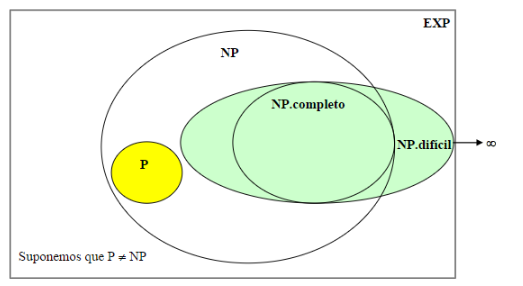
\includegraphics[scale=0.5]{images/CapturaClasificacion.PNG} 
			\end{center} 
		\end{figure}
		
	\end{frame}
	
	
	
	
	\section{Definición 3-DM}
	
	\begin{frame}{}
		\begin{center}
			\Huge{\textbf{3-DM}}				
		\end{center}
	\end{frame}
	
	
	\begin{frame}{Definición 3- Dimensional Matching I}
		\begin{block}{\textbf{Caso general}}
			X , Y , Z sean conjuntos finitos, disjuntos, y sea T un subconjunto de tripletas: 
			\\
			(x, y, z) /  x $\in$ X, y $\in$ Y , z $\in$ Z. 
		\end{block}
		
		\begin{block}{}
			Ahora M $\subseteq$ T es un conjunto, emparejamiento de 3 dimensiones, si se cumple lo siguiente: para cualquier par de tripletas distintas:
			
			\begin{center}
				($x_1$, $y_1$, $z_1$) $\in$  M 
				\\ ($x_2$, $y_2$, $z_2$) $\in$ M 
			\end{center}
			
			tenemos $x_1$  $\neq$  $x_2$, $y_1$  $\neq$  $y_2$, $z_1$  $\neq$  $z_2$.
		\end{block}
	\end{frame}
	
	
	\begin{frame}{Definición 3- Dimensional Matching II}
		\begin{block}{\textbf{Con otras palabras..}}
			Trata emparejar elementos de los 3 conjuntos(dimensiones x-y-z) de 3 en 3 sin que se repitan en ningún caso los elementos escogidos de cada conjunto.
		\end{block}
	\end{frame}
	
	
	\begin{frame}{Definición 3- Dimensional Matching III}
		\begin{block}{\textbf{Problema de decisión}}		
			Dado un conjunto T y un entero k, decidir si existe un 3-DM M $\subseteq$ T con $\mid$M$\mid$ $\geq$ k.
		\end{block}
		\begin{block}{}
			Sean X, Y y Z conjuntos disjuntos finitos y sea T un subconjunto de tripletas: 
			\\ (x, y, z) /  x $\in$ X, y $\in$ Y , z $\in$ Z. 
			\\ M $\subseteq$ T  es un emparejamiento 3-Dimensional si cumple que para cualquier par de tripletas:
			\begin{center}
				($x_1$, $y_1$, $z_1$) $\in$ M 
				\\($x_2$, $y_2$, $z_2$) $\in$ M
			\end{center}
			tenemos  $x_1$ $\neq$ $x_2$, $y_1$ $\neq$ $y_2$, $z_1$ $\neq$ $z_2$.
		\end{block}
	\end{frame}		
	
	
	\begin{frame}{Definición 3- Dimensional Matching IV}
		\begin{block}{\textbf{Con otras palabras..}}
			Trata de responder verdadero o falso, existe o no existe, que la cardinalidad de un conjunto de selecciones sea mayor o igual que un número dado (K).
		\end{block}
	\end{frame}
	
	
	\begin{frame}{Definición 3- Dimensional Matching V}
		\begin{block}{\textbf{Problema de optimización}}
			Dado un conjunto T , encontrar un juego de 3 dimensiones, M $\subseteq$ T que maximiza $\mid$M$\mid$.
		\end{block}	
		
		\begin{block}{}
			\begin{itemize}
				\item Dado que el problema de decisión descrito anteriormente NP-completo, este problema de optimización es NP-hard, y por lo tanto parece que no hay algoritmo de tiempo polinómico para la búsqueda de una coincidencia máxima 3-dimensional. 
				\item Sin embargo, existen algoritmos de tiempo polinómico eficientes para la búsqueda de un máximo coincidente bipartito (coincidencia máxima de 2 dimensiones), por ejemplo, el algoritmo de Hopcroft-Karp.
			\end{itemize}
		\end{block}
	\end{frame}
	
	
	\begin{frame}{Definición 3- Dimensional Matching VI}
		\begin{block}{\textbf{Con otras palabras..}}
			Trata de emparejar elementos de los 3 conjuntos(dimensiones x-y-z) de 3 en 3 sin que se repitan en ningún caso los elementos escogidos de cada conjunto, cumpliendo que la cardinalidad de los conjuntos seleccionados sea máxima.
		\end{block}
	\end{frame}
	
	
	\begin{frame}{Ejemplo 3- Dimensional Matching VII}
		\begin{block}{Ejemplo}
			Abajo se muestran emparejamientos de 3 dimensiones o elementos. 
			\begin{itemize}
				\item El conjunto X está marcado con puntos rojos
				\item Y está marcada con puntos azules
				\item Z está marcado con puntos verdes
			\end{itemize}
		\end{block}
		
		\begin{block}{}	
			\begin{itemize}
				\item La figura (a) muestra el conjunto T (zonas grises). 
				\item La figura (b) muestra un juego de 3 dimensiones M con $\mid$M$\mid$ = 2.
				\item La Figura (c) muestra un juego de 3 dimensiones M con $\mid$M$\mid$ = 3.
			\end{itemize}
		\end{block}
		
		\begin{center}
			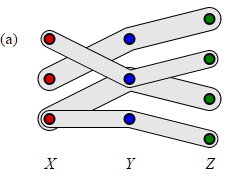
\includegraphics[scale=0.5]{images/CapturaA.PNG}
			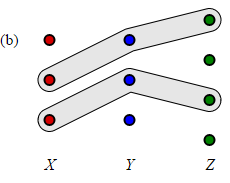
\includegraphics[scale=0.5]{images/CapturaB.PNG}
			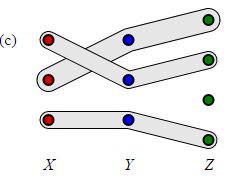
\includegraphics[scale=0.5]{images/CapturaC.PNG}
		\end{center}
		
	\end{frame}
	
	
	\begin{frame}{Ejemplo 3- Dimensional Matching}
		\begin{block}{}
			La coincidencia de M se ilustra en la figura (c) es un emparejamiento de 3 dimensiones máximo, es decir, se maximiza $\mid$M$\mid$. Las agrupaciones de las figuras (b) y (c) son máximos 3-DM, es decir, no pueden ser extendidos por la adición de más elementos de T.
		\end{block}
		
		\begin{center}
			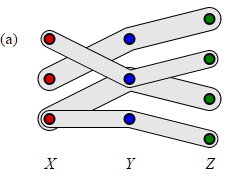
\includegraphics[scale=0.5]{images/CapturaA.PNG}
			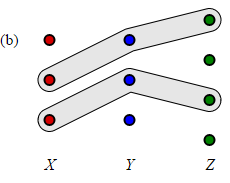
\includegraphics[scale=0.5]{images/CapturaB.PNG}
			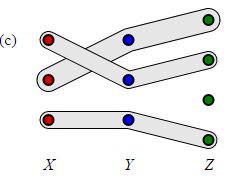
\includegraphics[scale=0.5]{images/CapturaC.PNG}
		\end{center}
	\end{frame}
	
	
	
	
	\section{Demostración 3-DM}
	
	\begin{frame}{Demostración 3DM es NP}
		
		\begin{block}{\textbf{3DM es NP}}
			Suponga que hay algún algoritmo no determinista que de alguna manera te devuelve una lista de n tripletas. Todo lo que debe suceder ahora es que hay que verificar en tiempo polinómico que las tripletas dadas son válidas, que es simple, ya que sólo se asegura que ninguna de las tripletas tienen el mismo valor en todas coordenada. Por lo tanto podemos concluir que 3DM está en NP.	
		\end{block}
		
	\end{frame}
	
	
	\begin{frame}{Demostración 3DM es NP-completo I}
		
		\begin{block}{\textbf{3SAT $\preceq$ 3DM}}
			Para probar que 3DM es NP-completo, tenemos que demostrar que 3SAT es reducible a 3DM.
			
		\end{block}	
		
		\begin{center}
			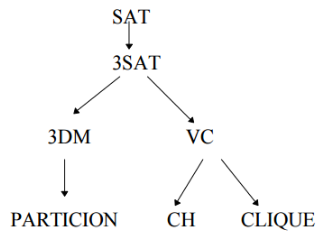
\includegraphics[scale=0.75]{images/Capturareduccion.PNG}
		\end{center}	
		
	\end{frame}
	
	
	\begin{frame}{Demostración 3DM es NP-completo II}
		\begin{block}{\textbf{Presentación del problema}}
			Sea $\alpha = C_1 \wedge, C_2 \wedge \dots \wedge C_{k-1}$ una instancia del 3SAT con variables $x_1, \dots, x_n$.
			Construiremos una instancia $I$ de 3DM de manera que $\alpha$ sea satisfactible si y sólo si $I$ tiene solución. Especificamos las tripletas de U en tres grupos: 
			\begin{itemize}
				\item El primer grupo se usa para \textbf{seleccionar una asignación verdadera}. 
				\item El segundo grupo se usa para \textbf{comprobar la satisfacción}. 
				\item El tercer grupo se utiliza de \textbf{recolección de basura}.
			\end{itemize}
			
		\end{block}
	\end{frame}
	
	\begin{frame}{Demostración 3DM es NP-completo III}
		
		\begin{block}{\textbf{Grupo 1: Seleccionar asignación verdadera}}
			Para cada variable $x_i, 1 \leq i < n$, tenemos $2k$ tripletas:
			
			$G_{i1} = {(a_{ij}, x_{ij}, b_{ij}), (b_{ij} , \overline x_{ij}, a_{i,(j+1)mod k}), 0 \leq j < k}$
			
			
		\end{block}
		No va a haber otra tripleta conteniendo los puntos $a_{ij}$ ni $b_{ij}, (1 \leq i \leq n, 0 \leq j < k)$. Las tripletas del grupo uno se pueden visualizar de la siguiente forma (k = 3):
		\begin{center}
			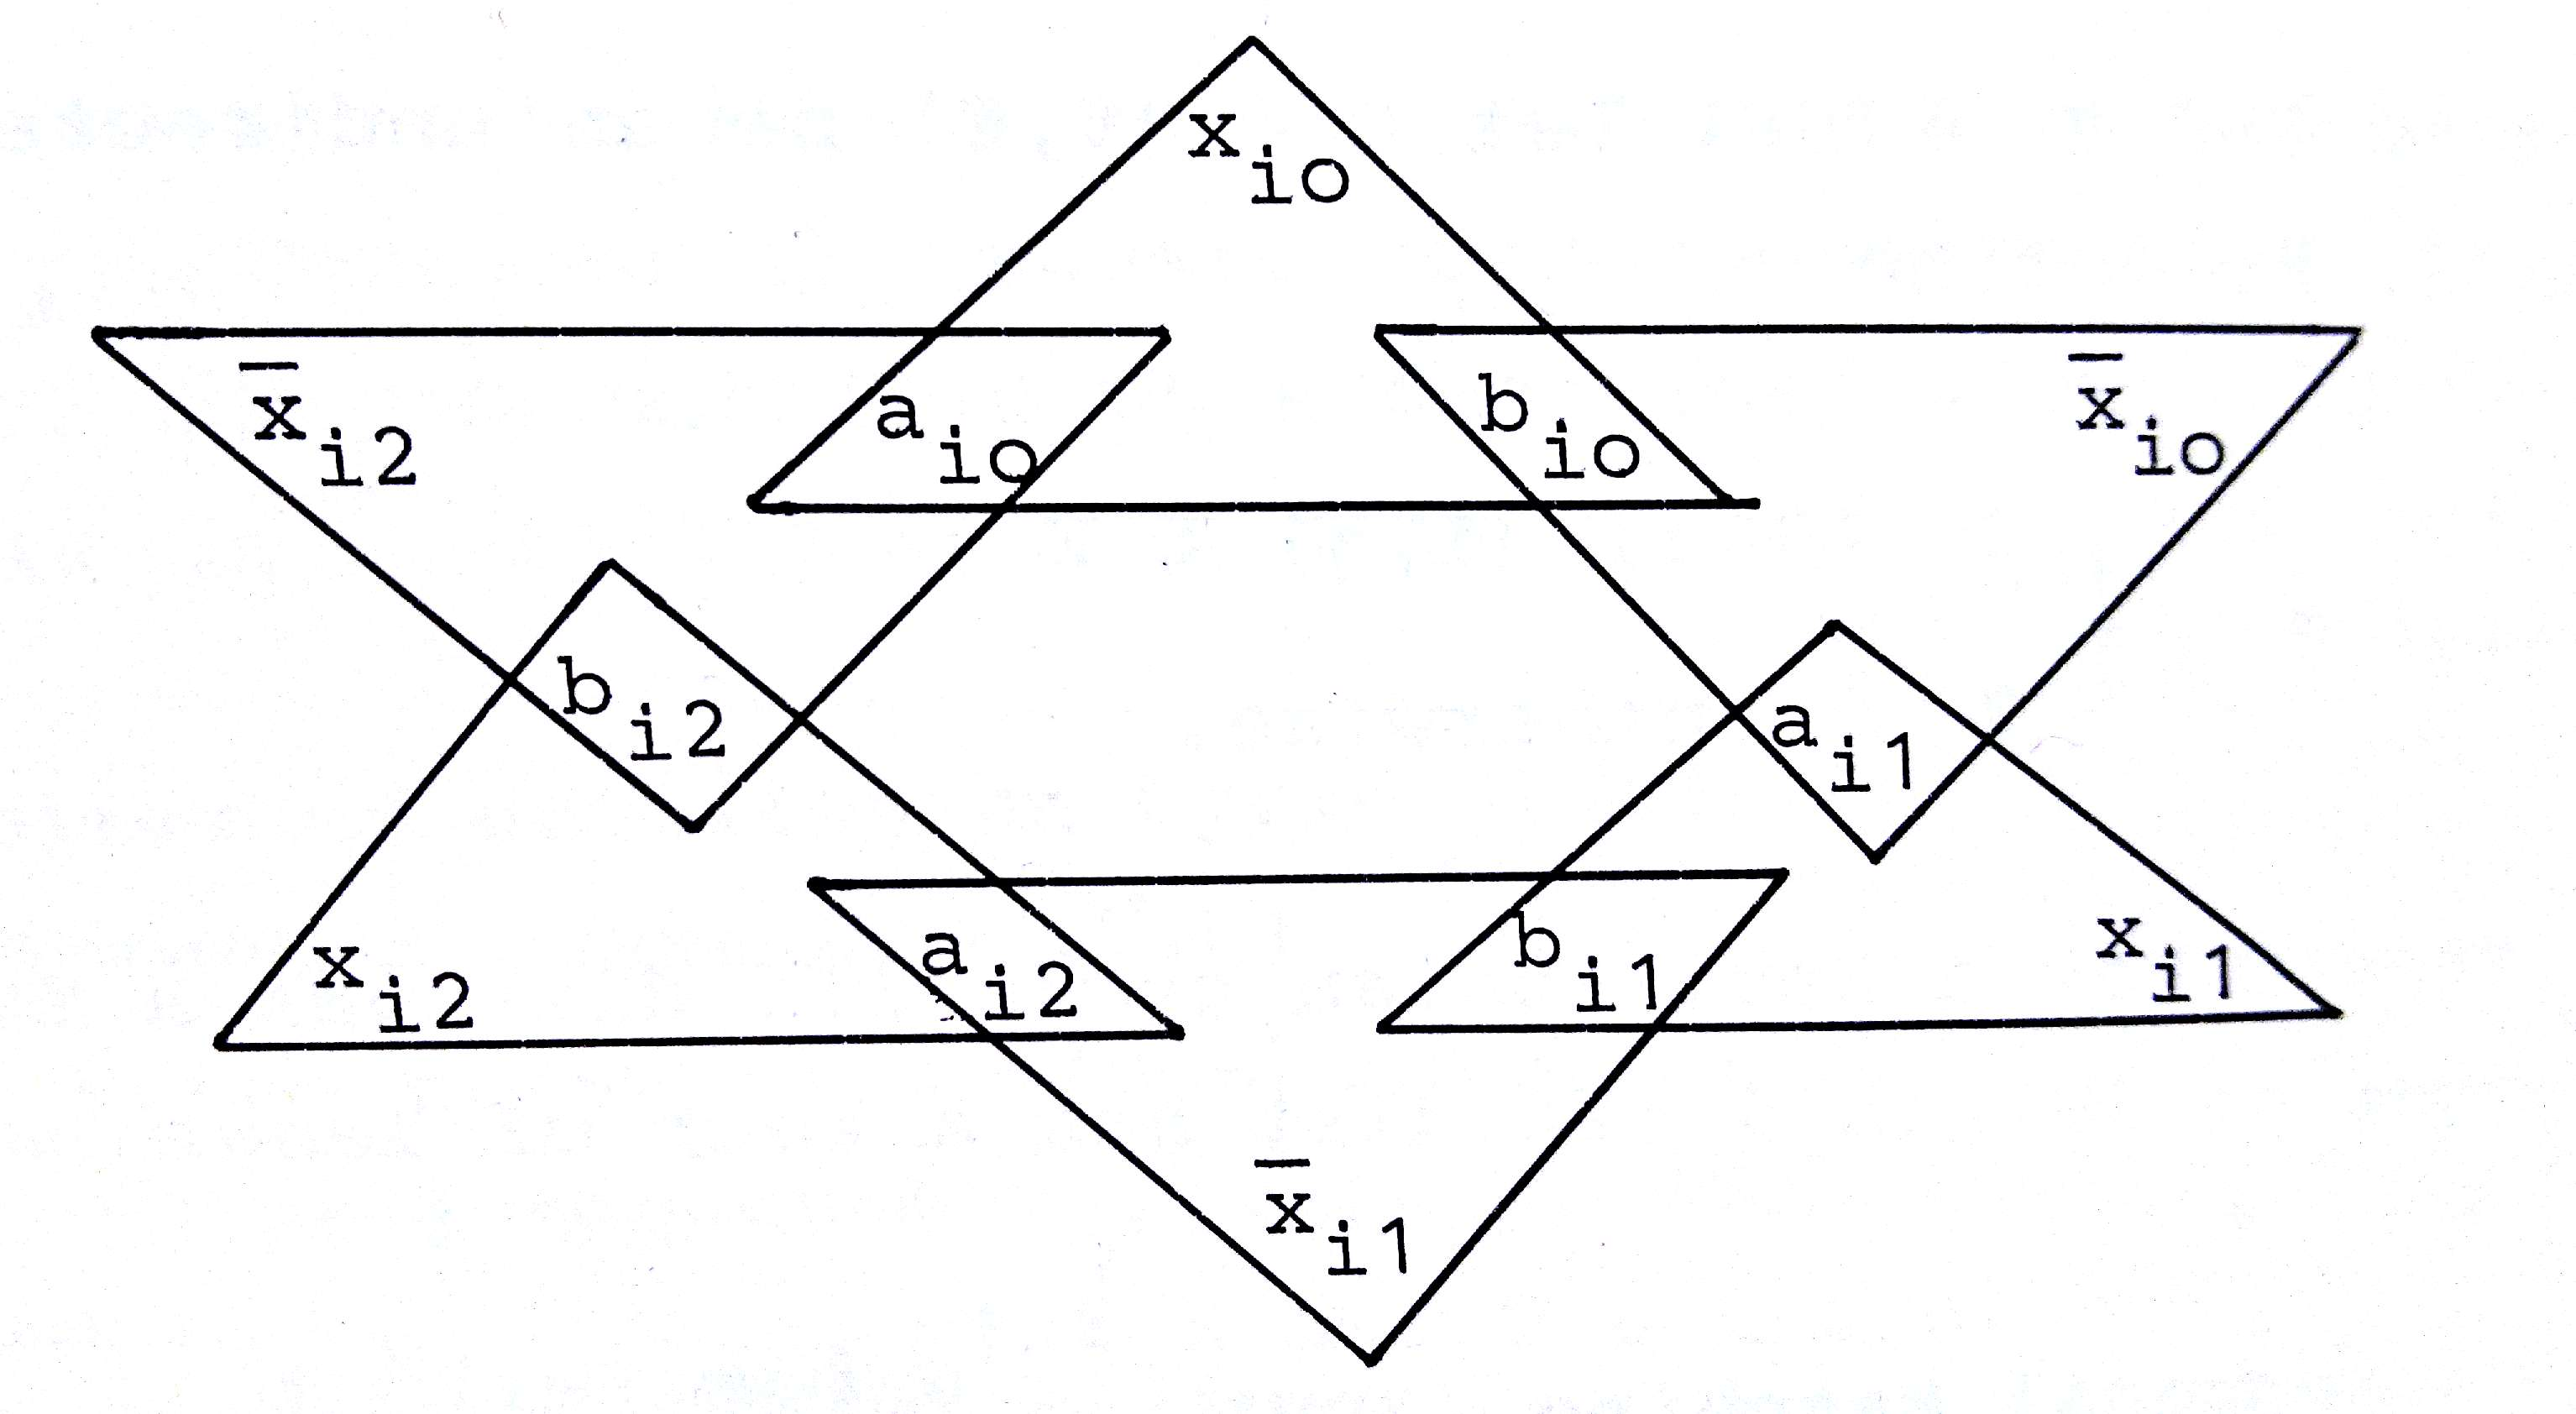
\includegraphics[scale=0.068]{images/grupo1.jpg}
		\end{center}
	\end{frame}
	
	\begin{frame}{Demostración 3DM es NP-completo IV}
		
		\begin{block}{\textbf{Grupo 1: Seleccionar asignación verdadera}}
			Hay exactamente dos formas de cubrir los puntos $a_{ij}, b_{ij}, 0 \leq j < k$, usando las tripletas en $G_{i1}$:
			\\Dejar todos los $x_{ij}$ descubiertos y cubrir los $\overline x_{ij}, 0 \leq j < k$ ($x_i$ es true)
			\\Dejar los puntos $\overline x_{ij}$ descubiertos y cubrir los $x_{ij}, 0 \leq j < k$ ($x_i$ es falso). 
			\\De esta forma, las tripletas de $G_{i1}$ arreglan una asignación verdadera.
			
		\end{block}
		
		\begin{center}
			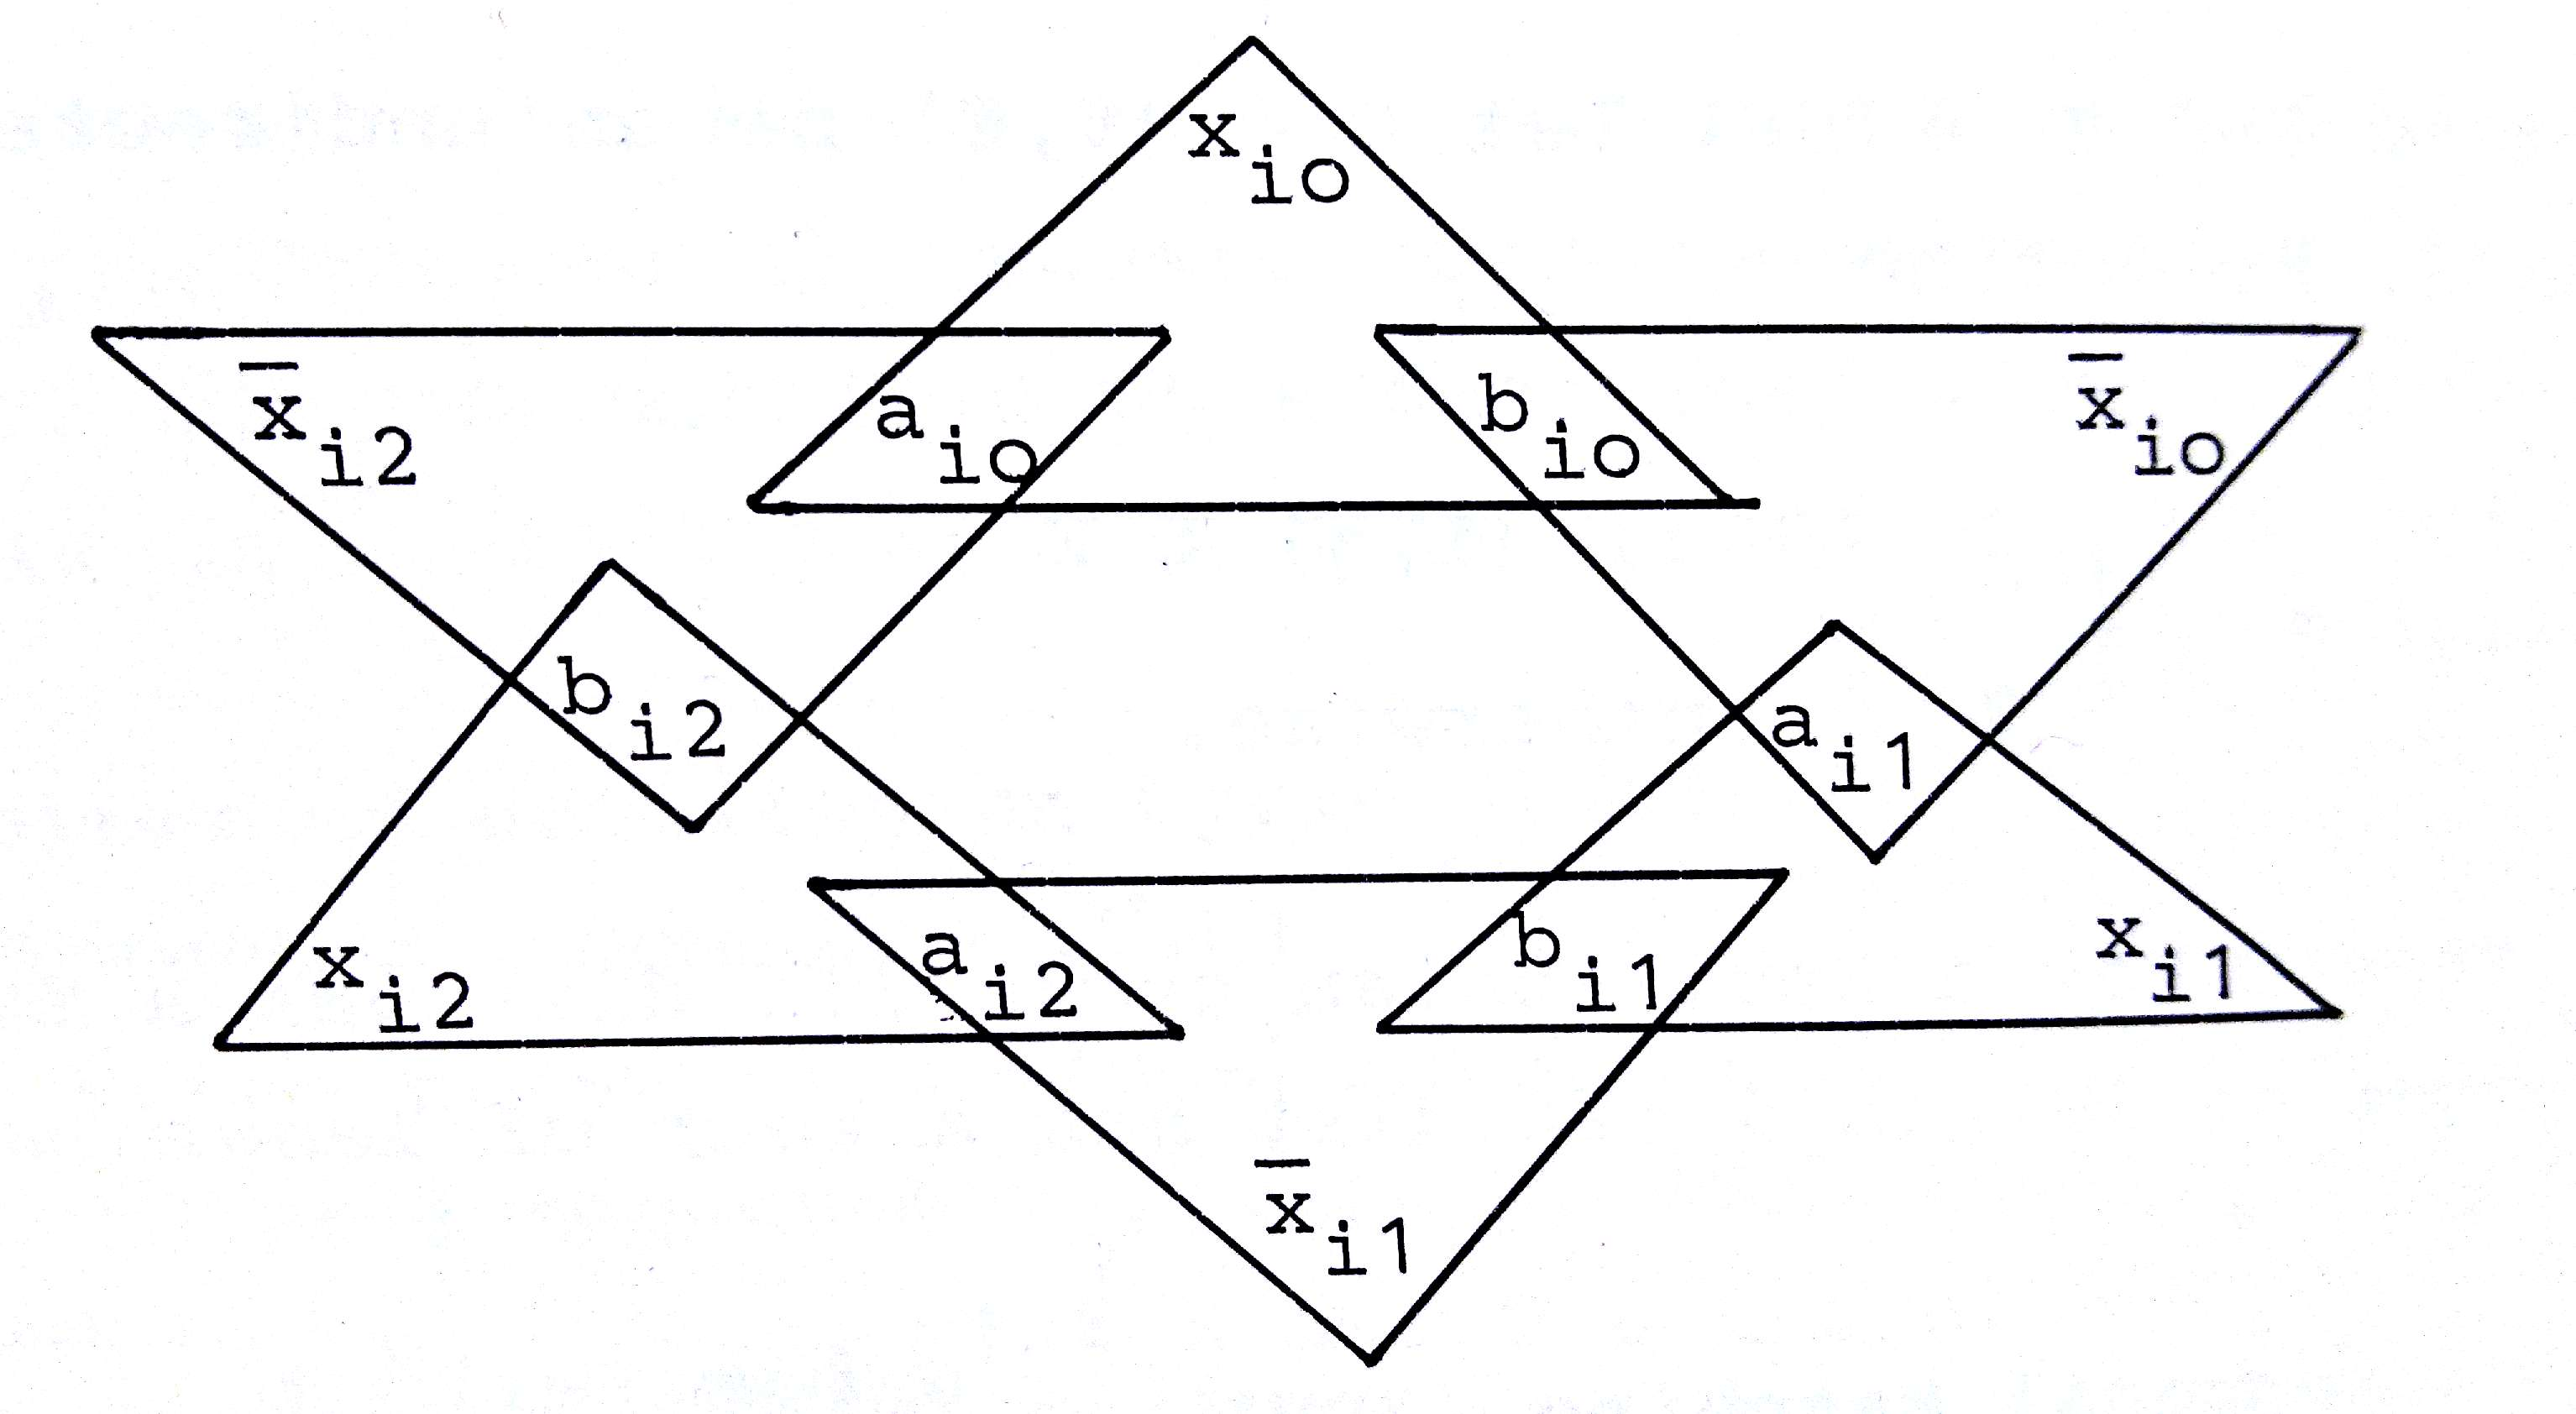
\includegraphics[scale=0.068]{images/grupo1.jpg}
		\end{center}	
		
	\end{frame}
	
	
	\begin{frame}{Demostración 3DM es NP-completo V}
		
		\begin{block}{\textbf{Grupo 2: Comprobación de satisfacción}}
			Para toda cláusula $C_j, 0 \leq j < k$, tenemos las tripletas ($S_1, \lambda, S_2$) para cada literal $\lambda$ que 
			aparezca en la cláusula.
			No hay más tripletas que contengan los puntos $S_2$ y $S_2$. \\ 
			
		\end{block}
		\begin{block}{}
			
			Supongamos ahora que los puntos del grupo 1 ya están seleccionados.
			Los puntos $S_!$ y $S_2$ pueden cubrirse si y sólo si hay una $i$ tal que $x_{ij}$  (ó $\overline x_{ij})$ aparece en 
			$C_j$ y se queda descubierta por los puntos del grupo 1. 
			\\Así, los puntos \textbf{$S_1$, $S_2$, $0 \leq j < k$, 
				pueden ser cubiertos} si y sólo si la asignación verdadera especificada en las tripletas del grupo 1 \textbf{satisfacen $\alpha$}
			
		\end{block}
	\end{frame}
	
	
	\begin{frame}{Demostración 3DM es NP-completo VI}
		
		\begin{block}{\textbf{Grupo 3: Recolección de basura}}
			En este punto, hemos construido una instancia de $I$ de $3DM$ a partir de $\alpha$ con la siguiente propiedad: 
			\\Si $\alpha$ es \textbf{insatisfactible}, \textbf{no puede haber matching completo} en $I$. 
			\\Si $\alpha$ es \textbf{satisfactible}, hay una manera de seleccionar las tripletas del grupo 1 y 2 de manera que los puntos 
			$a_{ij}, b_{ij} , S_1$ y $S_2$	\textbf{están todos cubiertos} y exactamente $nk - k = (n-1) k$ de los puntos $x_{ij}, x_{ij}$
			están descubiertos.	
			
		\end{block}
		
		\begin{block}{}
			Para completar el cubrimiento, añadimos en el grupo 3 las tripletas: \\
			{($h_r, x_{ij}, g_r)$/ $1 \leq r \leq (n-1)k$, $1 \leq i \leq n$, $0 \leq j \leq k$}
		\end{block}
	\end{frame}
	
	
	\begin{frame}{Demostración 3DM es NP-completo VI}
		
		\begin{block}{}
			 $Z$ = \{$x_{ij}, \overline x_{ij}$/ $1 \leq i \leq n, 1 \leq, j, \leq k$\}
			 
			 $X$ = \{$A \bigcup S_1 \bigcup H$\}
			 
			 $Y$ = \{$B \bigcup S_2 \bigcup G$\}
			
		\end{block}
		\begin{block}{\textbf{Conclusión}}
			Ahora es fácil ver que las instancias $I(\alpha)$ de $3DM$ definidas anteriormente pueden ser construidas en tiempo 
			polinomial dado $\alpha$ y sabiendo que ese $\alpha$ es satisfactible si y sólo si $I(\alpha)$ permite una coincidencia
			completa. 
			
		\end{block}
		
		\begin{block}{}
			Esto demuestra que $SAT(3) \leq 3DM$
		\end{block}
		
	\end{frame}
	
	
	\begin{frame}{Comparación con matching bipartito}
		
		\begin{block}{\textbf{2 Dimensional Matching}}
			Un 2 Dimensional Matching se puede definir de una manera completamente análoga. Sean X e Y  conjuntos finitos, disjuntos, y T  subconjunto de formado por parejas (x,y). 
		\end{block}
	
		\begin{block}{}
			Ahora M  $\subseteq$ T es un 2 Dimensional Matching, si se cumple lo siguiente: 
			\\Para dos pares distintos:
			\begin{center}
				($x_1$, $y_1$) $\in$  M 
				\\($x_2$, $y_2$) $\in$  M
			\end{center}
			tenemos $x_1$ $\neq$  $x_2$ y $y_1$  $\neq$  $y_2$.
		\end{block}	
				
	\end{frame}


	\begin{frame}{Comparación con matching bipartito}
		
			\begin{block}{}
				En el caso de coincidencia de 2-dimensional, el conjunto T se puede interpretar como el conjunto de bordes en un grafo bipartito G = ( X,  Y,  T), donde cada borde en T se conecta un vértice en X a un vértice en Y . 
			\end{block}	
		
			\begin{block}{}
				2-DM es entonces un emparejamiento a partir del grafo G, es decir, un conjunto de aristas no adyacentes por parejas.
			\end{block}
		
	\end{frame}


	\begin{frame}
		\begin{block}{}
			Por lo tanto 3-DM se puede interpretar como una generalización de matchings a hypergrafos (una generalización de un grafo en el que un borde puede unirse a cualquier número de vértices):
		\end{block}
		\begin{block}{}
			los conjuntos de X, Y y Z contienen los vértices, cada elemento de T es un hyperedge, y el conjunto de M consta de bordes no adyacentes por pares (bordes que no tienen un vértice común). En caso de coincidencia de 2 dimensiones, tenemos Y = Z.
		\end{block}
	\end{frame}
	

	\begin{frame}{Referencias}
		
		\begin{block}{}
			\begin{itemize}{}
				\item \url{http://www.math.cmu.edu/~af1p/Texfiles/PLANAR3DM.pdf}
				\item \url{https://sites.google.com/site/theuniverseofproblems/problems/3-dimensional-matching}
				\item \url{https://en.wikipedia.org/wiki/3-dimensional\_matching}
				\item \url{http://users.dsic.upv.es/~esanchis/clases/ALT/tema3.PDF}
				\item \url{http://studylib.es/doc/535768/01-medidas-de-complejidad}
				\item \url{https://www.cs.cmu.edu/~ckingsf/bioinfo-lectures/3dm.pdf}
				\item \url{http://npcomplete.owu.edu/tag/3dm/}
				\item \url{http://courses.cs.vt.edu/cs5114/spring2009/lectures/lecture24-np-complete-problems.pdf}
			\end{itemize}
		\end{block}
		
	\end{frame}


	\begin{frame}{}
	\begin{center}
			\textbf{Diego Luis Afonso} - alu0100825657@ull.edu.es 
	\end{center}
	\begin{center}
			\textbf{Daniel Daher Pérez} - alu0100811933@ull.edu.es
	\end{center}
	\begin{center}
		\textbf{Cristina Tosco González} - alu0100821338@ull.edu.es
	\end{center}
	\begin{center}
		\textbf{Alberto Antonio Sarabia Suárez} - alu0100734676@ull.edu.es
	\end{center}
	\begin{center}
		\textbf{Daniel Antonio Fernández Pérez} - alu0100812534@ull.edu.es
	\end{center}
	\end{frame}


\end{document}